\section{What energy alone gives the capacity}\label{sec:energy-capacity}

Before asking for new inequalities, it is worth knowing what the always-available information
provides. For unforced Navier--Stokes this is the energy bound $\|u(t)\|_{L^2}\le\|u_0\|_{L^2}$.
This section shows that energy gives a valid capacity, that this capacity grows too fast to
certify DIV, and that a tempting sharper bound fails for the full subgrid port.

\subsection{The energy bound}

By \eqref{eq:closure}, with $v=G_ju$ and $w=H_ju$,
\[
y_j=\Delta_j\mathcal P\nabla\cdot F,\qquad F=v\otimes v-u\otimes u=-(v\otimes w+w\otimes v+w\otimes w).
\]
The output is a finite Fourier sum over the $O(2^{3j})$ frequencies of shell $j$, each carrying one
derivative of size $O(2^j)$, and each Fourier coefficient of $F$ is bounded by $\|F\|_{L^1}$ up to
the normalization of the box. Cauchy--Schwarz therefore gives
\begin{equation}\label{eq:shell-l1}
\|\Delta_j\mathcal P\nabla\cdot F\|_{L^2}\ \le\ C\,2^{5j/2}\,\|F\|_{L^1}.
\end{equation}
This uses only the finite output shell; no $L^1$ bound for the Leray projection is involved.
Since $\|F\|_{L^1}\le2\|v\|_{L^2}\|w\|_{L^2}+\|w\|_{L^2}^2\le 3\|u\|_{L^2}^2$,
\begin{equation}\label{eq:energy-power}
\|y_j\|_{L^2}\le C'\,2^{5j/2}\|u\|_{L^2}^2,\qquad
|p_j|\le C'\,2^{5j/2}\|u\|_{L^2}^2\,\|u_j\|_{L^2}\le C'\,2^{5j/2}\|u_0\|_{L^2}^3 .
\end{equation}

The last bound is an absolute bound on power, so for $u_0\ne0$ the choice
$\mathrm{Cap}(j)=C'2^{5j/2}\|u_0\|_{L^2}^3$ is a valid, positive capacity in the sense of WORK$\times$CAP.
(Zero data give the zero solution, which needs no capacity.) It is not an ICAP coefficient. Dividing the middle bound by
$\|u_j\|_{L^2}^2$ leaves a factor $1/\|u_j\|_{L^2}$, which can be arbitrarily large.

\paragraph{Consequence for DIV.}
For nonzero data and a constant work quantum, the comparison series $\sum_j\theta/(C'2^{5j/2}\|u_0\|_{L^2}^3)$
converges, so this capacity cannot certify DIV. By the discussion in \cref{sec:no-zeno-engine},
this proves neither that the minimal capacity has a convergent reciprocal series nor that a
sharper capacity is impossible. It shows only that energy alone does not close the chain.

\subsection{A shell-only bound fails for the full port}

A natural sharpening would bound the subgrid output by the strain and the shell itself:
\begin{equation}\label{eq:false-bound}
\|y_j\|_{L^2}\lesssim\|\nabla u\|_{L^\infty}\|u_j\|_{L^2},\qquad\text{hence}\qquad
|p_j|\lesssim\|\nabla u\|_{L^\infty}\|u_j\|_{L^2}^2 .
\end{equation}
Commutator estimates do give bounds of this type for selected high--low interactions. They cannot
cover the high--high part of $F$, which can feed a shell that is almost empty.

\begin{proposition}[Exact counterexample]\label{prop:sgs-counterexample}
On $(\R/2\pi\mathbb{Z})^3$ let $k=(4,0,0)$, $l=(-3,1,0)$, $q=k+l=(1,1,0)$, $a=(0,1,0)$, $b=(1,3,0)$,
$c=(1,-1,0)$, and for $\varepsilon>0$
\[
u_\varepsilon(x)=a\cos(k\cdot x)+b\cos(l\cdot x)-\varepsilon\,c\sin(q\cdot x).
\]
Then $u_\varepsilon$ is smooth, zero-mean and divergence-free, $\|\nabla u_\varepsilon\|_{L^\infty}$ is
bounded uniformly for $0<\varepsilon\le1$, and at $j=0$
\[
y_0(u_\varepsilon)=-\tfrac32\,c\sin(q\cdot x),\qquad
p_0=\tfrac32\,\varepsilon\,|\T^3|,\qquad \|u_{\varepsilon,0}\|_{L^2}^2=\varepsilon^2|\T^3| .
\]
Hence $p_0/\|u_{\varepsilon,0}\|_{L^2}^2=3/(2\varepsilon)$ is unbounded, and neither inequality in
\eqref{eq:false-bound} holds with a constant independent of the field.
\end{proposition}

\begin{proof}
The three modes are divergence-free because $k\cdot a=l\cdot b=q\cdot c=0$. On this box $G_0$ keeps
the modes with $|k|<2$, so $G_0u_\varepsilon=u_{\varepsilon,0}=-\varepsilon c\sin(q\cdot x)$ and the modes $k$, $l$
are eliminated. The retained field has no self-advection, and every interaction of the retained
mode with an eliminated mode lands outside $\pm q$. The only contribution to shell $0$ comes from
the product of the two eliminated modes. The $q$-component of $(h\cdot\nabla)h$, with
$h=a\cos(k\cdot x)+b\cos(l\cdot x)$, equals $-\tfrac12\bigl((a\cdot l)\,b+(b\cdot k)\,a\bigr)\sin(q\cdot x)
=-\tfrac12(1,7,0)\sin(q\cdot x)$. Removing its component along $q$ leaves
$\tfrac32c\sin(q\cdot x)$, so $\Delta_0\mathrm{NL}(u_\varepsilon)=\tfrac32c\sin(q\cdot x)$ while
$\Delta_0\mathrm{NL}(u_{\varepsilon,0})=0$. By \eqref{eq:closure} this gives $y_0=-\tfrac32c\sin(q\cdot x)$; pairing with $u_{\varepsilon,0}$ and using $|c|^2=2$ gives $p_0$ and the shell energy.
\end{proof}

\begin{figure}[t]
  \centering
  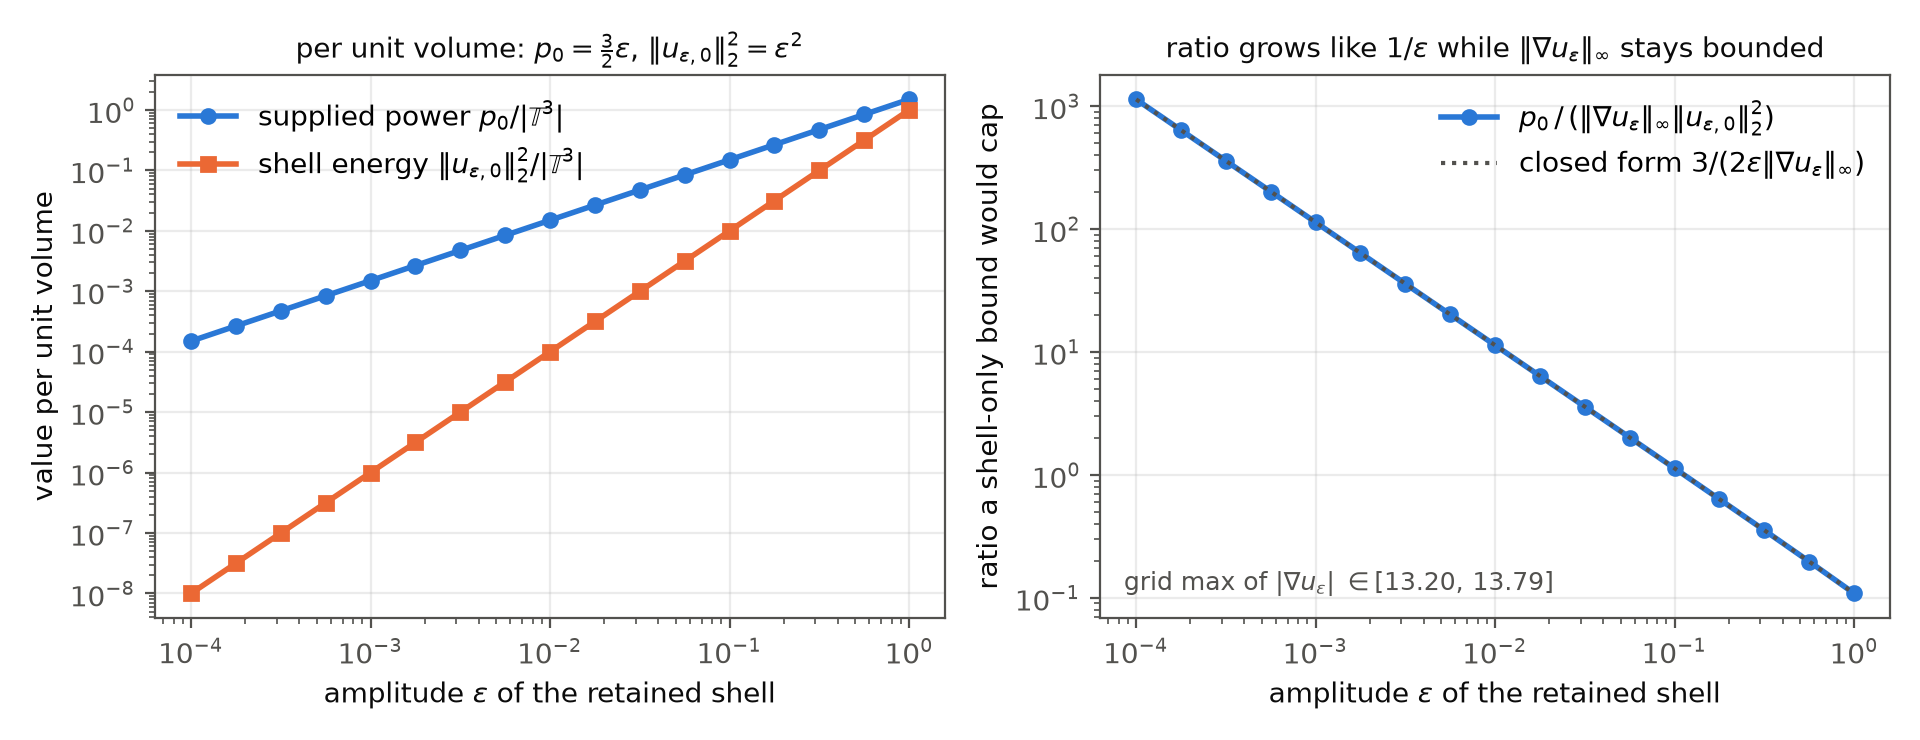
\includegraphics[width=\linewidth]{../python/artifacts/paper/ns_sgs_shell_counterexample.png}
  \caption{\textbf{The shell-only bound fails.} The field of \cref{prop:sgs-counterexample},
  evaluated with the repository's de-aliased pseudo-spectral nonlinearity on a $24^3$ grid
  (integrals normalized by volume). Left: the supplied power falls like $\varepsilon$ while the shell
  energy falls like $\varepsilon^2$. Right: the ratio that \eqref{eq:false-bound} would bound grows
  like $1/\varepsilon$, while the grid maximum of $|\nabla u_\varepsilon|$ stays between 13.2 and 13.8.
  The computed output matches $-\tfrac32c\sin(q\cdot x)$ to $4\times10^{-15}$.}
  \label{fig:sgs-counterexample}
\end{figure}

Each $u_\varepsilon$ is a smooth initial datum with a local smooth Navier--Stokes solution, so the
counterexample lives in the instantaneous domain of the actual port. It refutes one specific
estimate. It is not a no-go result for cumulative bounds over time windows, for the nonlinear
packaged history class, or for other functionals. The finite no-go theorem of
\cref{sec:no-go-icap} concerns a different, discrete statement and is unaffected.
